\documentclass[a4paper]{article}
\usepackage[14pt]{extsizes} % для того чтобы задать нестандартный 14-ый размер шрифта
\usepackage[utf8]{inputenc}
\usepackage[russian]{babel}
\usepackage{setspace,amsmath}
\usepackage[left=20mm, top=15mm, right=15mm, bottom=15mm, nohead, footskip=10mm]{geometry} 
\usepackage[pdftex]{graphicx}
\usepackage{amsfonts}
\usepackage{listings}
\usepackage{amssymb}
\usepackage{color}
\usepackage{textcomp}
\definecolor{listinggray}{gray}{0.9}
\definecolor{lbcolor}{rgb}{0.9,0.9,0.9}
\usepackage{amsthm}% настройки полей документа
\lstset{
    language=java,
    upquote=true,
    aboveskip={1.5\baselineskip},
    columns=fullflexible,
    showstringspaces=false,
    extendedchars=true,
    breaklines=true,
    showtabs=false,
    showspaces=false,
    showstringspaces=false,
    identifierstyle=\ttfamily,
    keywordstyle=\color[rgb]{0,0,1},
    commentstyle=\color[rgb]{0.133,0.545,0.133},
    stringstyle=\color[rgb]{0.627,0.126,0.941},
}

\newtheorem{definition}{Определение}
 
\begin{document} % начало документа

 Рассмотрим передаточную функцию:
$K(x)\frac{1}{(1+\tau_{p1}x)(1+\tau_{p2}x)} = \frac{1}{1+(\tau_{p1}+\tau_{p2})x + \tau_{p1}\tau_{p2}x^2}$\\
Введем обозначения:
$a = \tau_{p1}+\tau_{p2}$
$b = \tau_{p1}\tau_{p2}$\\
Рассмотрим первое условие теоремы:\\
$Re(\varkappa K(ix)-K(ix)^*\varepsilon K(ix)-[K(ix)-ix]^*\tau[K(ix)+ix])\geq\delta$\\
Подставим, рассматриваемую передаточную функцию в условие теоремы:\\
$K(ix)=\frac{1}{1+ax + bx^2}=\frac{1-bx^2-iax}{(1-bx^2)^2 + a^2x^2}$\\\\
$K(ix)^*K(ix)=\frac{1}{(1-bx^2)^2 + a^2x^2}$\\
$\frac{\tau b^2x^6 + (\tau a^2-2*\tau*b)x^4 + (\varkappa*b+\tau)x^2 + (\varkappa-\varepsilon-\tau)}{(1-bx^2)^2 + a^2x^2}\geq\delta$\\
В результате преобразований условие теоремы принимает следующий вид:\\
$\tau b^2t^3 + (\tau a^2-2 \tau b - \delta b^2)t^2 + (\varkappa b+\tau-\delta a^2 + 2\delta b)t + (\varkappa-\varepsilon-\tau-\delta) \geq 0 $\\
Где $t=x^2$\\
Второе условие теоремы имеет вид: \\
$4\varepsilon\delta > \nu^2\varkappa^2$\\
$\frac{4\varepsilon\delta}{\varkappa^2} > \nu^2$\\
Хотим найти max  $\nu$. Для этого будем искать максимум $\frac{4\varepsilon\delta}{\varkappa^2}$\\\\

1. Очевидно, что  $\varkappa - \varepsilon - \tau - \delta \geq 0$\\
$\varkappa \geq \varepsilon+\tau+\delta $\\
$\varkappa^2 \geq \varepsilon^2 + \tau^2 + \delta^2 + 2\varepsilon\tau + 2\varepsilon\delta + 2\tau\delta$\\
$2 -(\frac{2\varepsilon^2}{\varkappa^2} + \frac{2\delta^2}{\varkappa^2} + \frac{2\tau^2}{\varkappa^2} +\frac{4\varepsilon\tau}{\varkappa^2} + \frac{4\tau\delta}{\varkappa^2}) \geq \frac{4\varepsilon\delta}{\varkappa^2}$\\
$2 > \frac{4\varepsilon\delta}{\varkappa^2}$\\\\

2. Так как $\varkappa - \varepsilon - \tau - \delta \geq 0$, то $ \varepsilon \leq \varkappa - \tau - \delta$. Для максимизации функции $\frac{4\varepsilon\delta}{\varkappa^2}$ возьмем $\varepsilon = \varkappa - \tau - \delta$\\
Тогда первое условие теоремы принимает вид:\\
$\tau b^2t^2 + (\tau a^2-2 \tau b - \delta b^2)t + (\varkappa b+\tau-\delta a^2 + 2\delta b) \geq 0 $\\
И будем искать максимум следующей функции: $\frac{4\varepsilon\delta}{\varkappa^2} = \frac{4(\varkappa - \tau - \delta)\delta}{\varkappa^2} = 4\frac{\delta}{\varkappa} - 4\frac{\delta}{\varkappa}\frac{\tau}{\varkappa} - 4\frac{\delta^2}{\varkappa^2} = 4z-4z_1z - 4z^2$, \\
где $z_1 = \frac{\tau}{\varkappa}, z = \frac{\delta}{\varkappa}$\\
Опустим константу, так как она не влияет на максимизацию функции. Будем рассматривать $f(z) = z-z_1z - z^2$, как функцию от $z$ с параметром $z_1$.\\
Очевидно, что максимум этой функции достигается при $z_{max} = \frac{1-z_1}{2}$ и $f(z_{max}) = \frac{(1-z_1)^2}{4}$\\
Для того, что бы выполнялось первое условие теоремы возможны 2 случая: отрицательный дискриминант или оба корня меньше 0.\\\\

Рассмотрим дискриминант:\\ 
$D = (\tau a^2-2 \tau b - \delta b^2)^2 - 4\tau b^2 (\varkappa b+\tau-\delta a^2 + 2\delta b)$\\
Разделим на $\varkappa^2 > 0$\\
$\frac{D}{\varkappa^2} = (\frac{\tau}{\varkappa} a^2-2 \frac{\tau}{\varkappa}  b - \frac{\delta}{\varkappa}  b^2)^2 - 4\frac{\tau}{\varkappa}  b^2 (b+\frac{\tau}{\varkappa} -\frac{\delta}{\varkappa}  a^2 + 2\frac{\delta}{\varkappa}  b) = (z_1 a^2-2 z_1  b - z  b^2)^2 - 4z_1  b^2 (b+z_1  - z  a^2 + 2z b) = (z_1 a^2-2 z_1  b - \frac{1-z_1}{2} b^2)^2 - 4z_1  b^2 (b+z_1  - \frac{1-z_1}{2}  a^2 + 1-z_1 b)=z_1^2(-4b^2-2a^2b^2+4b^3+(a^2-2b+\frac{b^2}{2})^2)-z_1(\frac{b^4}{2}+2b^3-a^2b^2+4b^2) + \frac{b^4}{4}$\\\\

Множество допустимых значений $z_1$ состоит из тех $z_1$ для которых:   $D < 0$ или $D \geq 0$ и $x_2 < 0$, где $x_2$ наибольший корень.\\
Рассмотрим $D_1 = (\frac{b^4}{2}+2b^3-a^2b^2+4b^2)^2-b^4(-4b^2-2a^2b^2+4b^3+(a^2-2b+\frac{b^2}{2})^2)$. Реализуется случаи:\\\\

 2.1 $D_1 <  0$ и $(-4b^2-2a^2b^2+4b^3+(a^2-2b+\frac{b^2}{2})^2) > 0$\\
 Пусть $\varkappa = 1$, тогда $D \geq 0$, значит $M = \max\limits_{\frac{(\tau a^2-2 \tau b - \delta b^2)+\sqrt{D(z_1)}}{2\tau b^2}  \leq 0  }{|1-z_1|}$\\
 $f_{max} = \frac{(1-M)^2}{4}$\\\\
 
  2.2 $D_1 \geq 0$ и $(-4b^2-2a^2b^2+4b^3+(a^2-2b+\frac{b^2}{2})^2) > 0$\\
 Пусть $\varkappa = 1$, тогда корни уравнения $D = 0$ будут $d_{1,2} = \frac{(\frac{b^4}{2}+2b^3-a^2b^2+4b^2)\pm\sqrt{D_1}}{2(-4b^2-2a^2b^2+4b^3+(a^2-2b+\frac{b^2}{2})^2)}$\\
 При $z_1\in(d_1, d_2)$ $ D < 0$, значит $M_1 = \max\limits_{z_1\in(d_1, d_2)}{|1-z_1|}$\\
 При $z_1\in(-\inf, d_1]\cup[d_2, +\inf)$ $ D \geq 0$, значит $M_2 = \max\limits_{\frac{(\tau a^2-2 \tau b - \delta b^2)+\sqrt{D(z_1)}}{2\tau b^2}  \leq 0  }{|1-z_1|}$\\
 $M = max\{ M_1, M_2\}$\\
 $f_{max} = \frac{(1-M)^2}{4}$\\
 
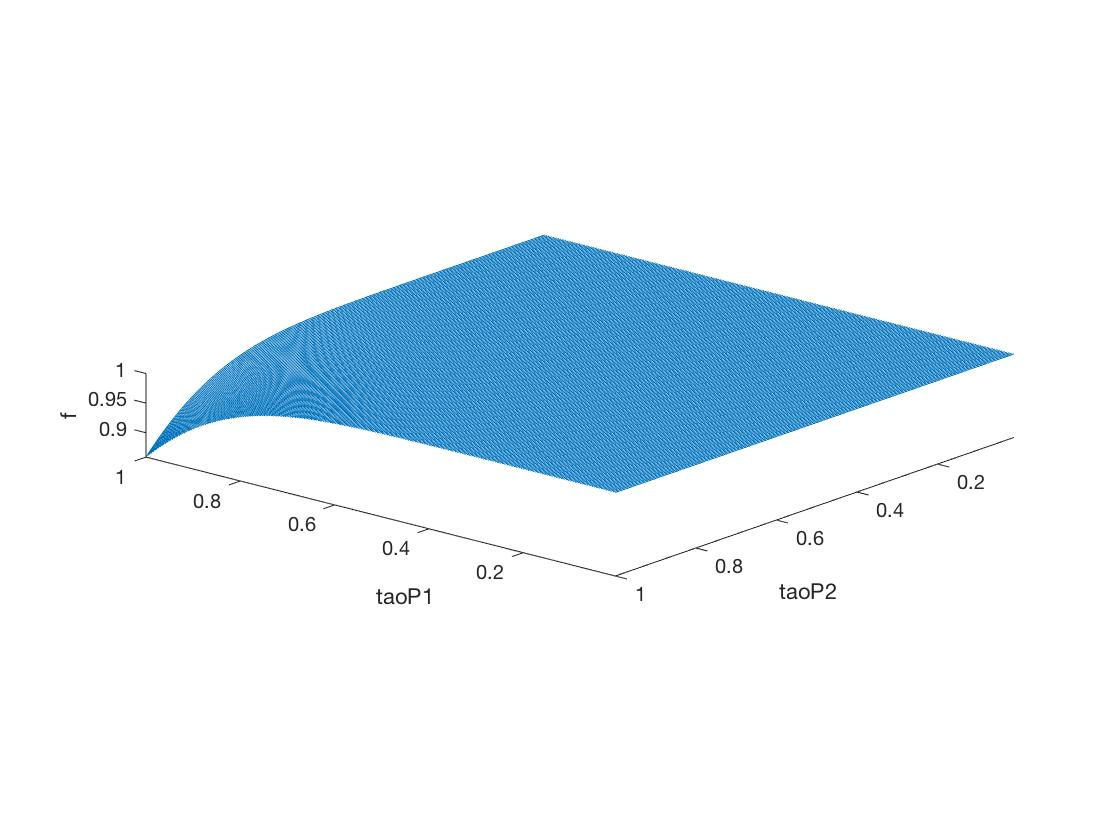
\includegraphics[width=12cm]{Images/filter1.jpg}
 
\end{document}  % КОНЕЦ ДОКУМЕНТА !